\section{Angle Uncertainty related to Converters}
\label{sec:uncertainty}

This section addresses the uncertainty of harmonic current phasors, especially phase angles, related to the typical industrial load with a 6-pulse line-commutated converter (LCC) as shown in Fig. \ref{fig:topo_indust_LCC}. The modeling method integrates steady-state harmonic state-space (HSS) model into Monte Carlo simulation (MCS), which enables the assessment of uncertainty propagation from key circuit parameters to harmonic phase angle.

First, a steady-state HSS model of LCC is established, which captures the mutual coupling among the harmonic phasors and their dependence on key passive parameters, namely the commutation inductance $L_{ac}$ on the AC side and the smoothing inductance $L_{dc}$ on the DC side. Then, the parameterized model is integrated into a stochastic assessment framework. The key parameters are modeled as random variables with realistic bounds. The MCS is applied to genetate probability distributions of harmonic phasors. Finally, the marginal probability density functions (PDFs) are fitted using the best-fit method, and the Gaussian copula correlation matrix of harmonic phase angles is obtained to indicate the inter-harmonic correlation.

\begin{figure}[ht!]
\centering
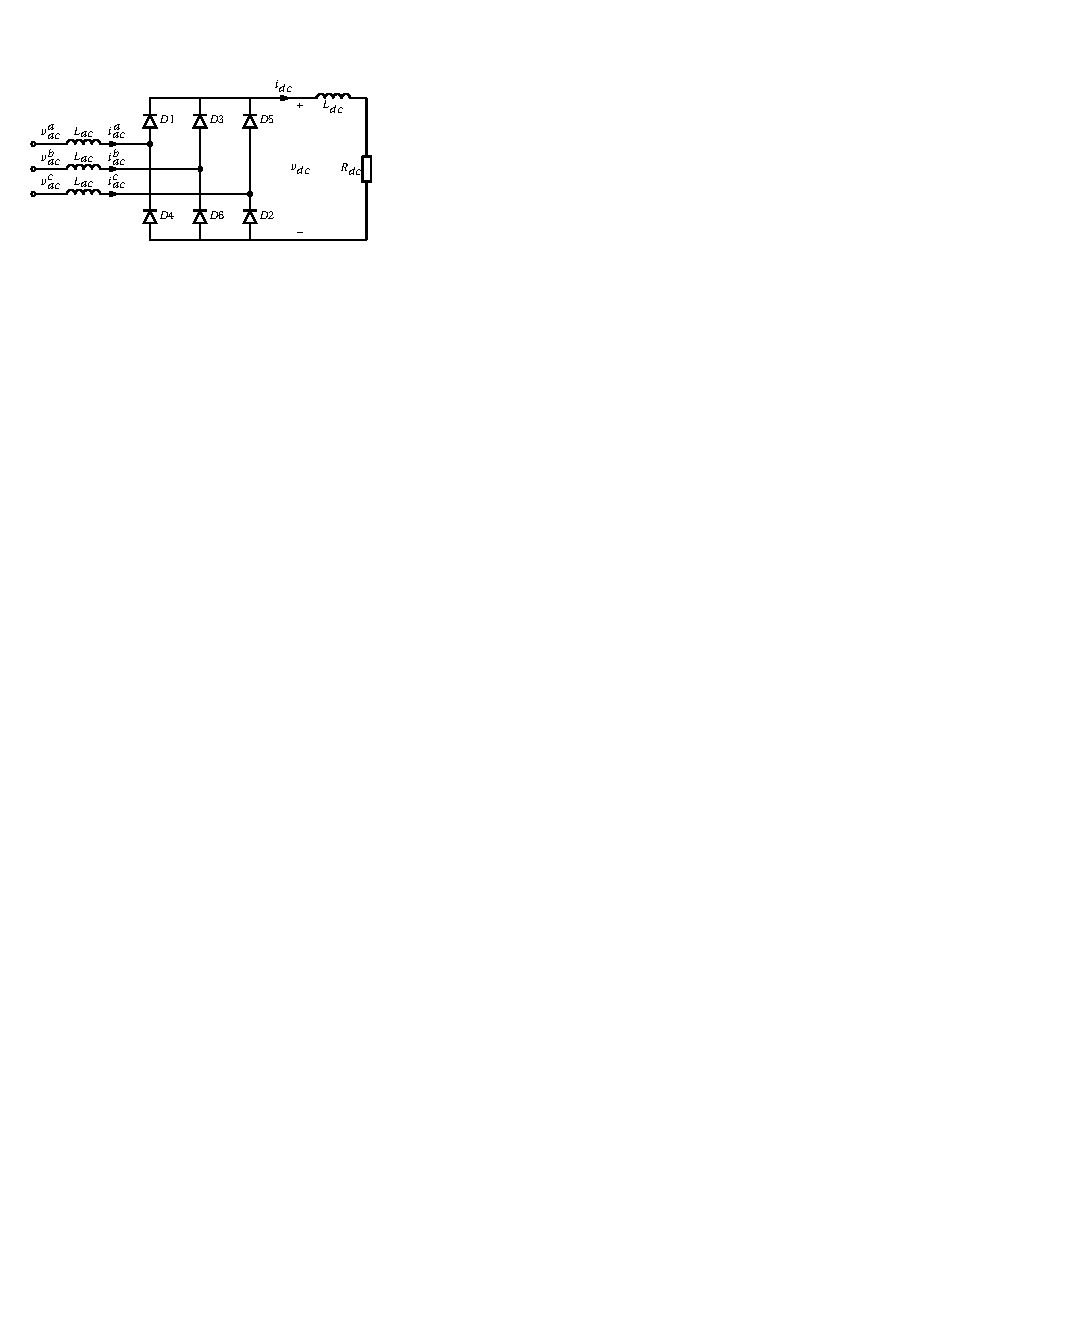
\includegraphics[width=0.8\columnwidth]{figures/topo_indust_LCC.pdf}
\caption{6-pulse line-commutated converter}
\label{fig:topo_indust_LCC} 
\end{figure}

\subsection{Steady-State Harmonic Model} 
Inherent frequency coupling is the key feature of converter-generated harmonics, which decide the recombination of harmonic phasors. Therefore, the accurate HSS model is built here to capture the nature commutation and harmonic coupling of LCC converter.

The LCC converter operates periodically with sequential valve switching creating 12 switching states per fundamental cycle. Each state is governed by differential equations with time-varying coefficients representing circuit topology changes. The state equations for any switching state can be expressed using piecewise switching functions $S_{dc,ac}^{i}(t)$, $S_{dc}(t)$, and $S_{ac}^{i,j}(t)$ as:
\begin{IEEEeqnarray}{l}
    (S_{dc} L_{ac} + L_{dc}) \frac{di_{dc}}{dt} = \nonumber \\ S_{dc,ac}^{a} v_{ac}^a + S_{dc,ac}^{b} v_{ac}^b + S_{dc,ac}^{c} v_{ac}^c - R_{dc} i_{dc}, \label{eq:idc_t} \\
    % L_{ac} \frac{di_{ac}^a}{dt} - S_{dc,ac}^{a} L_{ac} \frac{di_{dc}}{dt} = \nonumber \\ S_{ac}^{a,a} v_{ac}^a + S_{ac}^{a,b} v_{ac}^b + S_{ac}^{a,c} v_{ac}^c, \label{eq:iac_t} \\
    L_{ac} \frac{di_{ac}^i}{dt} - S_{dc,ac}^{i} L_{ac} \frac{di_{dc}}{dt} = \nonumber \\ S_{ac}^{i,a} v_{ac}^a + S_{ac}^{i,b} v_{ac}^b + S_{ac}^{i,c} v_{ac}^c, \label{eq:iac_t}
\end{IEEEeqnarray}
where $v_{ac}^{i}$ and $i_{ac}^{i}$ denote AC-side voltage and current, the superscript $i \in \{a, b, c\}$ represents the three phases, $v_{dc}$ and $i_{dc}(t)$ are DC-side voltage and current. All these switching functions are parameterized by the commutation angle $\mu$ in steady state.

The HSS model transforms these time-domain equations into frequency domain through three operations: (1) Fourier series expansion of state variables $x(t) = \sum_{h=-N_h}^{N_h} X_h e^{jh\omega_1 t}$, (2) frequency-domain differentiation $d\mathbf{X}/dt \leftrightarrow \mathbf{Z}_{\Omega}\mathbf{X}$ where $\mathbf{Z}_{\Omega} = j\omega_1 \cdot \text{diag}(h)$, and (3) Toeplitz convolution matrices representing time-domain multiplication: $y(t) = S(t)x(t) \Leftrightarrow \mathbf{Y} = \mathbf{S}_{conv}\mathbf{X}$. The resulting unified system relates current harmonics $\mathbf{I} = [\mathbf{I}_{ac}^a, \mathbf{I}_{ac}^b, \mathbf{I}_{ac}^c]^T$ to voltage harmonics $\mathbf{U} = [\mathbf{V}_{ac}^a, \mathbf{V}_{ac}^b, \mathbf{V}_{ac}^c]^T$ through:
\begin{equation}
\mathbf{A}\mathbf{I} = \mathbf{B}\mathbf{U}
\end{equation}
where matrices $\mathbf{A}$ and $\mathbf{B}$ contain Toeplitz convolution structures explicitly capturing frequency coupling. The model is parameterized by commutation overlap angle $\mu$, and circuit inductances ($L_{ac}$, $L_{dc}$), providing a foundation for subsequent MSC and uncertainty quantification.

\subsection{Methodology for Uncertainty Quantification}
At the planning stage, the uncertainty on key parameters comes from the limited knowledge about the future integrated device, as well as manufacturing tolerances and operational variances. To account for these parameter uncertainties, the inductances $L_{ac}$ and $L_{dc}$ are modeled as random variables, and the MCS is used for assessment of uncertainty propagation.

\subsubsection{Realistic parameter uncertainty bounds}
The uncertainties on $L_{ac}$ and $L_{dc}$ are modeled using truncated normal distributions:
\begin{equation}
L_{ac} \sim \mathcal{N}_{\text{trunc}}(\mu_{L_{ac}}, \sigma_{L_{ac}}^2, L_{ac,\min}, L_{ac,\max})
\label{truncated_normal_lac}
\end{equation}
\begin{equation}
L_{dc} \sim \mathcal{N}_{\text{trunc}}(\mu_{L_{dc}}, \sigma_{L_{dc}}^2, L_{dc,\min}, L_{dc,\max})
\label{truncated_normal_ldc}
\end{equation}
which are constrained within physically realistic bounds determined by engineering trade-offs at the industrial load design stage:
\begin{itemize}
    \item \textit{AC-side inductance $L_{ac}$:} The upper bound $L_{ac,\max}$ is limited by acceptable commutation angle and voltage drop, while the lower bound $L_{ac,\min}$ ensures adequate harmonic suppression and safe short-circuit current.

    \item \textit{DC-side inductance $L_{dc}$:} The upper bound $L_{dc,\max}$ is limited by required dynamic response, size, and cost, while the lower bound $L_{dc,\min}$ ensures DC ripple stays within specifications to prevent equipment aging and process quality degradation.
\end{itemize}

The truncated normal distribution enforces physical bounds while maintaining mathematical tractability for Monte Carlo propagation.

\subsubsection{Monte Carlo simulation}
MCS approach is adopted, by which a set of 5000 random sample pairs $(L_{ac}, L_{dc})$ is generated using rejection sampling to meet the defined constraints. For each of the parameter samples, a HSS model is built and solved. The iterative process involves:
\begin{itemize}
    \item Recalculating the commutation angle $\mathsf{\mu}$ based on the sampled pair of parameters.
    \item Reconstructing time-periodic switching functions $S_{dc,ac}^{i}(t)$, $S_{dc}(t)$, and $S_{ac}^{i,j}(t)$ based on the updated commutation angle.
    % \item Reconstructing time-periodic switching functions $\mathbf{S}_{dc,ac,conv}^{i}$, $\mathbf{S}_{dc,conv}$, and $\mathbf{S}_{ac,conv}^{i,j}$ based on the updated commutation angle.
    \item Numerically solving the HSS equations to extract and store the magnitudes and phase angles of the AC-side harmonic currents of interest.
\end{itemize}

\subsection{Probability Density Function Fitting}
A case study is conducted based on a representative 6-pulse LCC unit, with nominal capacity of 1.25 MW and nominal line voltage of 380 V, which is connected to the 35 kV bus through a rectifier transformer with a ratio of 35 kV/400 V. 
For the AC-side commutation inductance, the truncation bounds are $L_{ac,\min} = 0.01$ mH and $L_{ac,\max} = 0.03$ mH, corresponding to transformer short-circuit voltage percentages ranging from $U_k = 5\%$ to $15\%$. For the DC-side smoothing inductance, the truncation bounds are $L_{dc,\min} = 0.05$ mH and $L_{dc,\max} = 0.35$ mH.

Fig.\ref{fig:harmonic_phasors_CI_LacLdc} shows the harmonic phasor distribution of each characteristic harmonic, caused by parameter uncertainty. In each harmonic phasor distribution plot, the red one represents the phasor with mean magnitude and mean phase angle, while the blue ones represent the phasors within the 95\% confidence intervals (CI). The results indicate that: 1) the harmonic phasors at different frequencies exhibit mutual dependency; 2) higher orders of harmonics display progressively larger phaser angle variations and uncertainties.

\begin{figure*}[htb]
    \centering
    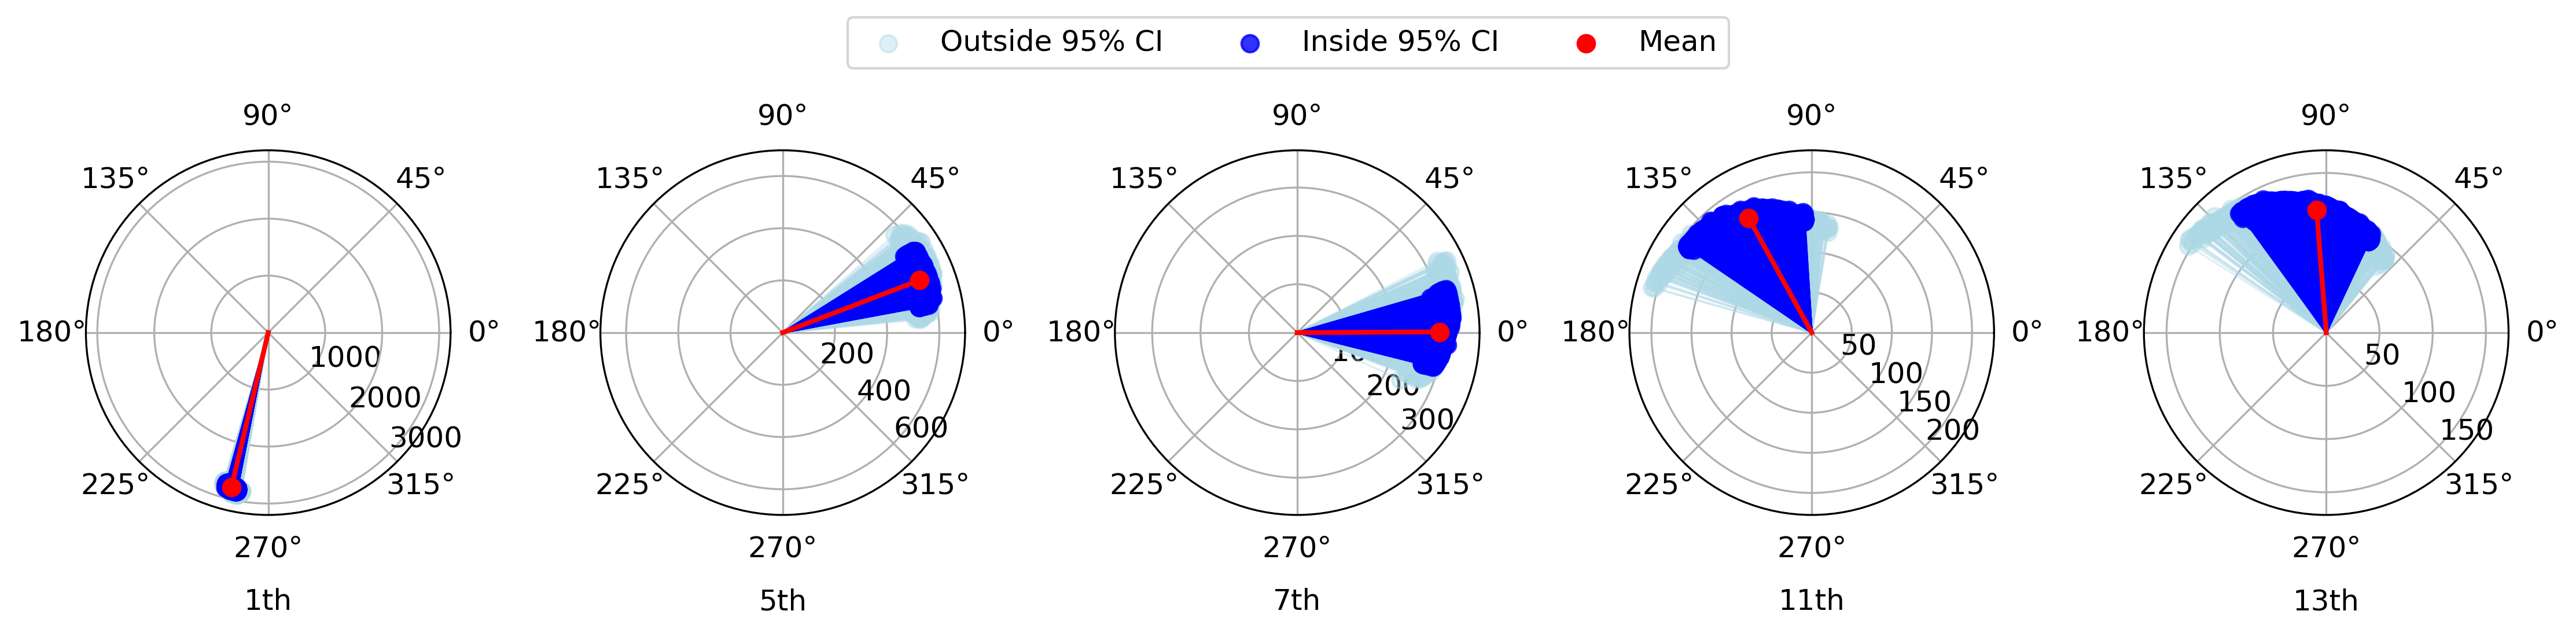
\includegraphics[width=0.8\textwidth]{figures/harmonic_phasors_CI_LacLdc.png}
    \caption{Harmonic phasor distributions caused by parameter uncertainty}
    \label{fig:harmonic_phasors_CI_LacLdc}
\end{figure*}

\begin{figure*}[htb]
    \centering
    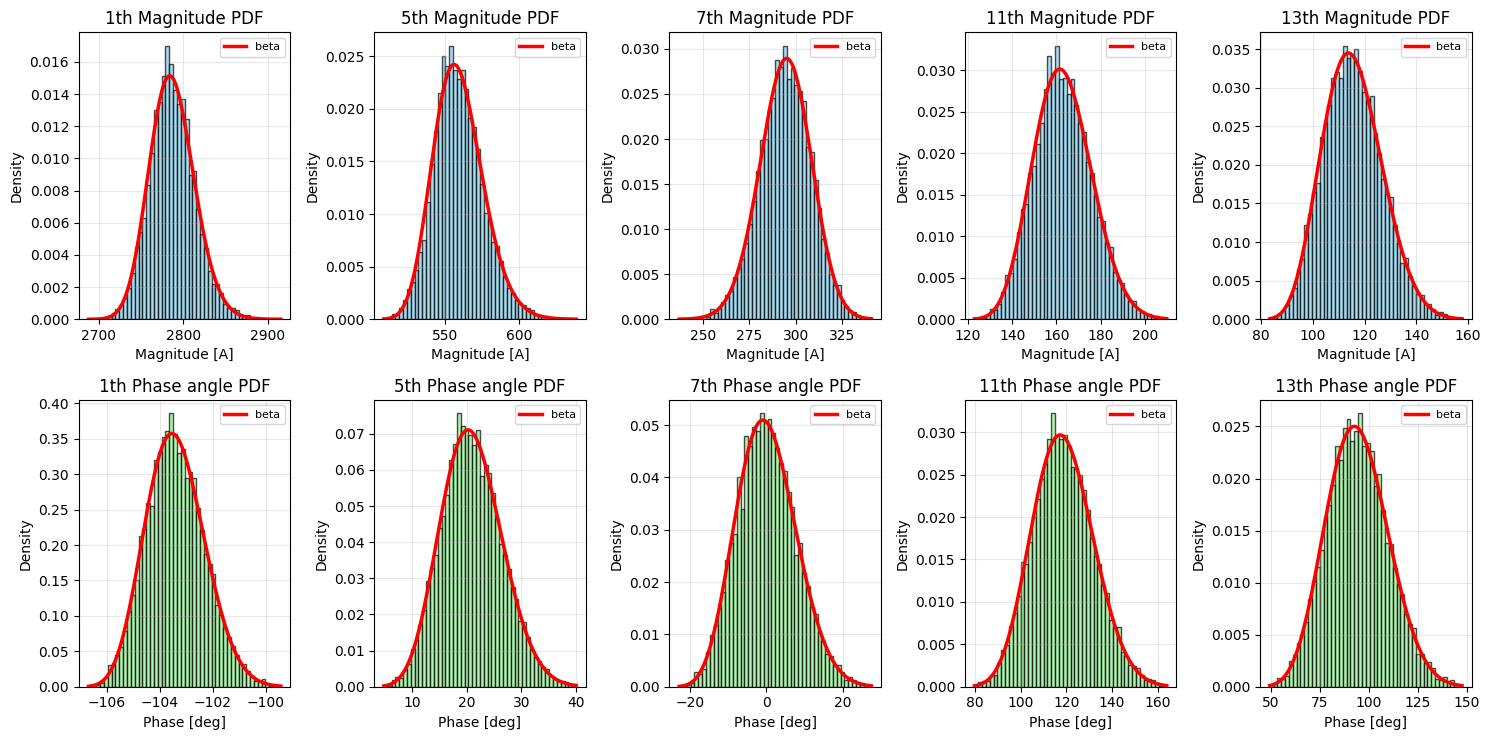
\includegraphics[width=0.8\textwidth]{figures/Bestfit_PDF.png}
    \caption{Harmonic phasor distributions with corresponding best-fit probability density functions.}
    \label{fig:Bestfit_PDF} 
\end{figure*}

\subsubsection{Marginal Distribution Fitting}
The marginal distributions of each harmonic component are modeled independently. The best-fit PDF for each harmonic magnitude and phase angle is fitted to the data obtained from MCS. The candidate distributions considered include Normal, Lognormal, Gamma, Logistic and Exponential distributions.

For each harmonic $i$, the marginal distribution $F_i(x_i)$ is estimated by fitting multiple parametric distributions and selecting the best-fit  distribution based on minimizing the Root Mean Squared Error (RMSE) between the cumulative distribution functions simulated and fitted. The best-fit results are illustrated in Fig.\ref{fig:Bestfit_PDF}, showing the histograms and the fitted PDFs of harmonic magnitudes and phase angles. Tables~\ref{tab:bestfit_phase} summarize the best-fit distributions and their estimated parameters for harmonic phase angles.

\begin{table}[h!] 
\centering
\caption{Best-Fit Distributions for Harmonic Phase Angles}
\label{tab:bestfit_phase}
\begin{tabular}{l l l l}
\hline
Order & Distribution & RMSE & Parameters \\
\hline
1st  & Gamma    & $1.2051 e^{-2}$ & $[ 69.9979, -112.6848,  0.1324]$ \\
5th  & Gamma    & $2.9152 e^{-3}$ & $[ 58.7859, -21.95,  0.7287]$ \\
7th  & Gamma    & $1.9757 e^{-3}$ & $[ 53.9904, -56.7056,  1.0529]$ \\
11th & Gamma    & $1.0178 e^{-3}$ & $[ 86.2671, -5.2519,  1.4358]$ \\
13th & Gamma    & $1.0509 e^{-3}$ & $[ 78.0513, -44.43,  1.7764]$ \\
\hline
\end{tabular}
\end{table}

The parameters of the Gamma distribution are given as $[k, \ell, \theta]$, where $k$ is the shape parameter, $\ell$ is the location parameter, and $\theta$ is the scale parameter.
% The PDF of Gamma Distribution, with shape = $k$, location = $\ell$, scale = $\theta$, is given by:
% \[
% f_{\Gamma}(x; k,\theta,\ell) =
% \frac{(x-\ell)^{k-1} e^{-(x-\ell)/\theta}}{\Gamma(k)\,\theta^{k}}, \quad x>\ell.
% ]

\subsubsection{Inter-Harmonic Dependency Analysis}
After getting the fitted marginal distributions, the correlation structure between different harmonic components is investigated. Correlation matrices, with Kendall's Tau correlation coefficients, are used to characterize the dependencies.

In Fig.~\ref{fig:Correlation_Matrix_Copula}, the phase angle correlation matrix $\mathbf{R}_{\text{phase}}$ exhibits very strong correlations ($\rho_{ij} \geq 0.97$), indicating distinct characteristics in the inter-harmonic dependency structure for phase angles. 

\begin{figure}[h!]
    \centering
    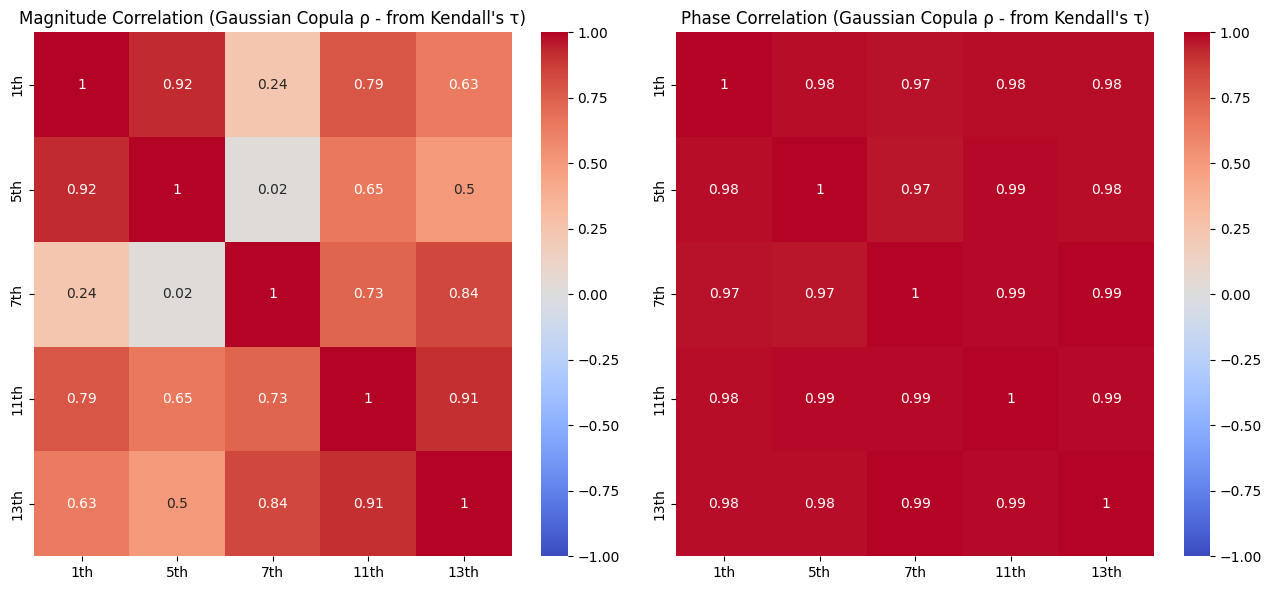
\includegraphics[width=\columnwidth]{figures/Correlation_Matrix_Copula.png}
    \caption{Gaussian copula correlation matrices for harmonic magnitudes and harmonic phase angles. (only phase angle is needed?)}
    \label{fig:Correlation_Matrix_Copula}
\end{figure}
